\documentclass[border=5pt]{standalone}
\usepackage[utf8]{inputenc}
\usepackage[T1]{fontenc}
\usepackage{tikz}
\usetikzlibrary{arrows.meta, positioning, shapes.geometric}
\begin{document}
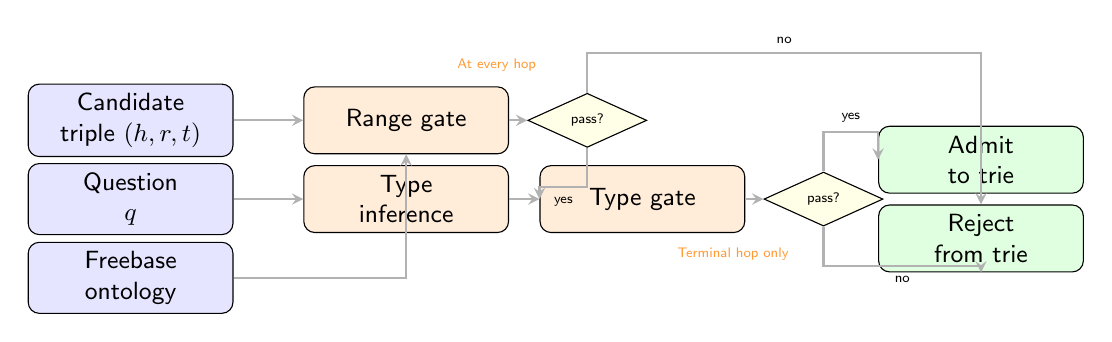
\begin{tikzpicture}[
  >=stealth, font=\sffamily,
  box/.style={draw, rounded corners, minimum width=2.6cm, minimum height=0.85cm,
    align=center, font=\sffamily\small},
  input/.style={box, fill=blue!10},
  gate/.style={box, fill=orange!15},
  output/.style={box, fill=green!12},
  arr/.style={->, thick, draw=gray!60},
  decision/.style={diamond, draw, aspect=2.2, minimum width=1.3cm,
    minimum height=0.65cm, align=center, font=\sffamily\tiny, fill=yellow!10},
]

  % Inputs
  \node[input] (triple) at (0, 1) {Candidate\\triple $(h,r,t)$};
  \node[input] (q) at (0, 0) {Question\\$q$};
  \node[input] (types) at (0, -1) {Freebase\\ontology};

  % Row 1: Range gate
  \node[gate] (rg) at (3.5, 1) {Range gate};
  \node[decision] (rgd) at (5.8, 1) {pass?};

  % Row 2: Type inference + Type gate (spread apart)
  \node[gate] (infer) at (3.5, 0) {Type\\inference};
  \node[gate] (tg) at (6.5, 0) {Type gate};
  \node[decision] (tgd) at (8.8, 0) {pass?};

  % Outputs (further right)
  \node[output] (admit) at (10.8, 0.5) {Admit\\to trie};
  \node[output] (reject) at (10.8, -0.5) {Reject\\from trie};

  % Connections - Row 1
  \draw[arr] (triple.east) -- (rg.west);
  \draw[arr] (types.east) -| (rg.south);
  \draw[arr] (rg.east) -- (rgd.west);

  % Range gate pass -> type gate
  \draw[arr] (rgd.south) -- ++(0,-0.5) -| node[pos=0.25, below, font=\sffamily\tiny] {yes} (tg.west);

  % Range gate fail -> reject
  \draw[arr] (rgd.north) -- ++(0,0.5) -| node[pos=0.25, above, font=\sffamily\tiny] {no} (reject.north);

  % Question -> type inference
  \draw[arr] (q.east) -- (infer.west);

  % Type inference -> type gate
  \draw[arr] (infer.east) -- (tg.west);

  % Type gate -> pass?
  \draw[arr] (tg.east) -- (tgd.west);

  % Type gate pass -> admit
  \draw[arr] (tgd.north) -- ++(0,0.5) -| node[pos=0.25, above, font=\sffamily\tiny] {yes} (admit.west);

  % Type gate fail -> reject
  \draw[arr] (tgd.south) -- ++(0,-0.5) -| node[pos=0.25, below, font=\sffamily\tiny] {no} (reject.south);

  % Annotations
  \node[font=\sffamily\tiny, text=orange!80] at (4.65, 1.7) {At every hop};
  \node[font=\sffamily\tiny, text=orange!80] at (7.65, -0.7) {Terminal hop only};

\end{tikzpicture}
\end{document}
